%%%%%%%%%%%%%%%%%%%%%%%%%%%%%%%%%%%%%%%%%%%%%%%%%%%%%%%%%%%%%%%%
%
% Documento con ejercicios resueltos de la 
% asignatura Análisis Matemático I.
% Doble Grado de Informática y Matemáticas.
% Universidad de Granada.
% Curso 2016/17.
% 
% 
% Colaboradores:
% Javier Sáez (@fjsaezm)
% Daniel Pozo (@danipozodg)
% Pedro Bonilla (@pedrobn23)
% Guillermo Galindo
% Antonio Coín (@antcc)
% Luis Rekteao (@Ludvins)
%
% Agradecimientos:
% Andrés Herrera (@andreshp) por la base para la plantilla.
% Mario Román (@M42) por la base para la portada.
%
% Sitio original:
% https://github.com/libreim/apuntesDGIIM/
%
% Licencia:
% CC BY 4.0 (https://creativecommons.org/licenses/by/4.0/)
%
%%%%%%%%%%%%%%%%%%%%%%%%%%%%%%%%%%%%%%%%%%%%%%%%%%%%%%%%%%%%%%%


%------------------------------------------------------------------------------
%   ACKNOWLEDGMENTS
%------------------------------------------------------------------------------

%%%%%%%%%%%%%%%%%%%%%%%%%%%%%%%%%%%%%%%%%%%%%%%%%%%%%%%%%%%%%%%%%%%%%%%%
% Plantilla básica de Latex en Español.
%
% Autor: Andrés Herrera Poyatos (https://github.com/andreshp) 
%
% Es una plantilla básica para redactar documentos. Utiliza el paquete  fancyhdr para darle un
% estilo moderno pero serio.
%
% La plantilla se encuentra adaptada al español.
%
%%%%%%%%%%%%%%%%%%%%%%%%%%%%%%%%%%%%%%%%%%%%%%%%%%%%%%%%%%%%%%%%%%%%%%%%%

%%%
% Plantilla de Trabajo
% Modificación de una plantilla de Latex de Frits Wenneker para adaptarla 
% al castellano y a las necesidades de escribir informática y matemáticas.
%
% Editada por: Mario Román
%
% License:
% CC BY-NC-SA 3.0 (http://creativecommons.org/licenses/by-nc-sa/3.0/)
%%%

%%%%%%%%%%%%%%%%%%%%%%%%%%%%%%%%%%%%%%%%
% Short Sectioned Assignment
% LaTeX Template
% Version 1.0 (5/5/12)
%
% This template has been downloaded from:
% http://www.LaTeXTemplates.com
%
% Original author:
% Frits Wenneker (http://www.howtotex.com)
%
% License:
% CC BY-NC-SA 3.0 (http://creativecommons.org/licenses/by-nc-sa/3.0/)
%
%%%%%%%%%%%%%%%%%%%%%%%%%%%%%%%%%%%%%%%%%


% Tipo de documento y opciones.
\documentclass[11pt, a4paper, titlepage]{article}


%---------------------------------------------------------------------------
%   PAQUETES
%---------------------------------------------------------------------------

% Idioma y codificación para Español.
\usepackage[utf8]{inputenc}
\usepackage[spanish, es-tabla, es-lcroman, es-noquoting]{babel}
\selectlanguage{spanish} 
%\usepackage[T1]{fontenc}

% Fuente utilizada.
\usepackage{courier}    % Fuente Courier.
\usepackage{microtype}  % Mejora la letra final de cara al lector.

% Diseño de página.
\usepackage{fancyhdr}   % Utilizado para hacer títulos propios.
\usepackage{lastpage}   % Referencia a la última página.
\usepackage{extramarks} % Marcas extras. Utilizado en pie de página y cabecera.
\usepackage[parfill]{parskip}    % Crea una nueva línea entre párrafos.
\usepackage{geometry}            % Geometría de las páginas.

% Símbolos y matemáticas.
\usepackage{amssymb, amsmath, amsthm, amsfonts, amscd}
\usepackage{upgreek}

% Otros.
\usepackage{enumitem}   % Listas mejoradas.
\usepackage{graphicx}


%---------------------------------------------------------------------------
%   OPCIONES PERSONALIZADAS
%---------------------------------------------------------------------------

% Redefinir letra griega épsilon.
\let\epsilon\upvarepsilon

% Formato de texto.
\linespread{1.1}            % Espaciado entre líneas.
\setlength\parindent{0pt}   % No indentar el texto por defecto.
\setlist{leftmargin=.5in}   % Indentación para las listas.

% Estilo de página.
\pagestyle{fancy}
\fancyhf{}
\geometry{left=3cm,right=3cm,top=3cm,bottom=3cm,headheight=1cm,headsep=0.5cm}   % Márgenes y cabecera.


%---------------------------------------------------------------------------
%   COMANDOS PERSONALIZADOS
%---------------------------------------------------------------------------

% Valor absoluto: \abs{}
\providecommand{\abs}[1]{\lvert#1\rvert}    

% Fracción grande: \ddfrac{}{}
\newcommand\ddfrac[2]{\frac{\displaystyle #1}{\displaystyle #2}}

% Texto en negrita en modo matemática: \bm{}
\newcommand{\bm}[1]{\boldsymbol{#1}}

% Línea horizontal.
\newcommand{\horrule}[1]{\rule{\linewidth}{#1}}


\newcommand{\R}{\mathbb{R}}


%---------------------------------------------------------------------------
%   CABECERA Y PIE DE PÁGINA
%---------------------------------------------------------------------------

% Cabecera del documento.
\renewcommand\headrule{
	\begin{minipage}{1\textwidth}
		\hrule width \hsize 
	\end{minipage}
}

% Texto de la cabecera.
\lhead{\subject: Ejercicios resueltos}  % Izquierda.
\chead{}            % Centro.
\rhead{DGIIM}    % Derecha.

% Pie de página del documento.
\renewcommand\footrule{                                 
	\begin{minipage}{1\textwidth}
		\hrule width \hsize   
	\end{minipage}\par
}

% Texto del pie de página.
\lfoot{}                                                 % Izquierda
\cfoot{}                                                 % Centro.
\rfoot{Página\ \thepage\ de\ \protect\pageref{LastPage}} % Derecha.


%---------------------------------------------------------------------------
%   ENTORNOS PARA MATEMÁTICAS
%---------------------------------------------------------------------------

% Nuevo estilo para los ejercicios
\newtheoremstyle{exercise-style} % Nombre del estilo.
{10pt}               % Espacio por encima.
{10pt}               % Espacio por debajo.
{}                   % Fuente del cuerpo.
{}                   % Identación.
{\bf}                % Fuente para la cabecera.
{.}                  % Puntuación tras la cabecera.
{.5em}               % Espacio tras la cabecera.
{\thmname{#1}\thmnumber{ #2}\thmnote{ (#3)}}     % Especificación de la cabecera (actual: nombre en negrita).

% Ejercicios
\theoremstyle{exercise-style}
\newtheorem*{ejer}{Ejercicio}

% Listas ordenadas con números romanos (i), (ii), etc.
\newenvironment{nlist}
{\begin{enumerate}
\renewcommand\labelenumi{(\emph{\roman{enumi})}}}
{\end{enumerate}}

% Teoremas, proposiciones y corolarios.
\theoremstyle{theorem-style}
\newtheorem*{nth}{Teorema}
\newtheorem*{nprop}{Proposición}
\newtheorem{ncor}{Corolario}

\newenvironment{rcases}
  {\left.\begin{aligned}}
  {\end{aligned}\right\rbrace}

%---------------------------------------------------------------------------
%   PÁGINA DE TÍTULO
%---------------------------------------------------------------------------

% Título del documento.
\newcommand{\subject}{Análisis Matemático I}

% Autor del documento.
\newcommand{\docauthor}{Doble Grado de Informática y Matemáticas}

% Título
\title{
  \normalfont \normalsize 
  \textsc{Universidad de Granada} \\ [25pt]    % Texto por encima.
  \horrule{0.5pt} \\[0.4cm] % Línea horizontal fina.
  \huge \subject\\  \Large Ejercicios resueltos\\ % Título.
  \horrule{2pt} \\[0.5cm] % Línea horizontal gruesa.
}

% Autor.
\author{\large{\docauthor}}

% Fecha.
\date{\vspace{-1.5em} \normalsize Curso 2016/17}


%---------------------------------------------------------------------------
%   COMIENZO DEL DOCUMENTO
%---------------------------------------------------------------------------
\begin{document}

\maketitle  % Título.


%--------------------------------------------
%   Topología de un espacio métrico
%--------------------------------------------
\section{Topología de un espacio métrico.}

\begin{ejer}
Dado el conjunto $A = \{ (x,y)\in \mathbb{R}^2: 0 < x \le 1 \}$, ¿es abierto?

\begin{proof}
Tenemos que comprobar si $A$ es abierto, es decir, si es cierto que\\
$\forall a \in A \ \ \exists s>0\ tal\ que\ B(a,s)\subset A$. Para ello, fijo $y \in \mathbb{R}$ y escojo $x_o = (1,y) \in A$. Además, tomo $s>0$ cualquiera. Veamos que hay puntos $z \in B(x_o, s)$ que no pertenecen a $A$.

Sea $\displaystyle z = (1 + \frac{s}{2}, y)$. Entonces, se tiene que $\displaystyle d(z,x_o)= \sqrt{\left(\frac{s}{2}\right)^2 + 0} = \frac{s}{2} < s$, y por tanto $z \in B(x_o,s)$.

Claramente $z\notin A$, pues $\displaystyle 1 + \frac{s}{2} > 1$. Así, concluimos que $z$ es un punto de $B(x_o,s)$ que no pertenece a $A$, por lo que $\displaystyle B(x_o,s) \not \subseteq A$, y $A$ no es abierto. \qedhere

%\textbf{@ Antonio Coín.}
\end{proof}

\end{ejer}

\section{Conexión.}
\begin{ejer} Dado el conjunto \emph{peine} de la siguiente forma, probar que es conexo:
\[
	P = (\{ 0\} \times (0,1]) \cup ((0,1] \times \{0\}) \cup (\{\frac{1}{n} : n \in \mathbb{N}\} \times (0,1)) 
\]

\begin{center}
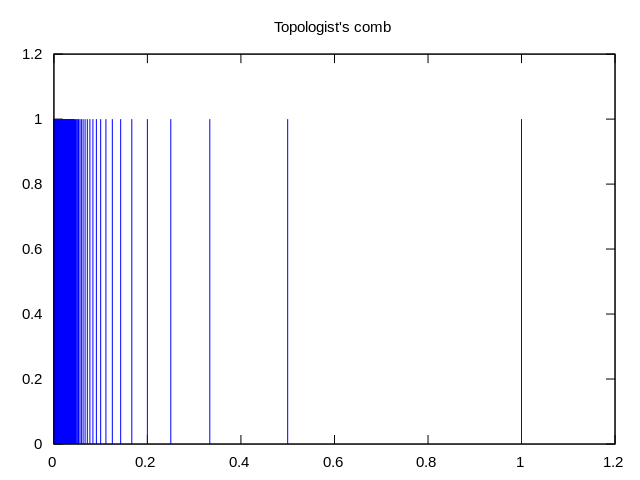
\includegraphics[scale=0.4]{imagenes/peine.png}
\end{center}

\begin{proof}
Para la demostración vamos a definir el siguiente conjunto:
\[
	S = ((0,1] \times \{0\}) \cup (\{\frac{1}{n} : n \in \mathbb{N}\} \times (0,1)) 
\]
Es decir, el mismo conjunto P quitandole el eje y. Siendo $\bar{S} = P \cup (0,0)$.
De esta forma tenemos:
\[
S \subset P \subset \bar{S}
\]

Para demostrar este ejercicio utilizaremos la siguiente proposición:\\

\begin{nprop}
Sea A un conjunto conexo, y B tal que $A \subset B \subset \bar{A} \implies B$ es conexo.
\end{nprop}

\begin{proof}
 Para la demostración probaremos su contrarecíproco, consistente en: B no es conexo $\implies$ A no es conexo.
 
B no es conexo $\implies \exists O,O'$ abiertos $: \begin{cases}
B \subset O\cup O'\\
O \cap B \cap O' = \emptyset\\
O \cap B \neq \emptyset \neq O' \cap B\\
\end{cases}$
 
 Debemos probar que los 3 resultados se cumplen para A. 
 
 1. $B \subset O \cup O' \implies A \subset B \subset O \cup O'$\\
 2. $B \cap (O\cap O') = \emptyset \implies \nexists x \in B$ tq $x \in O \cap O'$. \\
 Entonces $\forall x \in A \implies x \in B \implies x \not\in O \cap O'$\\
 3. $O \cap B \neq \emptyset \implies O\cap \bar{A} \neq \emptyset \implies O\cap (A\cup fr(A) \neq \emptyset \implies (O\cap A)\cup (O\cap fr(A)) \neq \emptyset$
 En este punto tenemos 3 posibilidades:\\
  - El primer elemento de la union es distinto del vacio, en cuyo caso hemos acabado.\\
  - Ambos elementos son distintos del vacio, en cuyo caso tambien queda demostrado.\\
  - El segundo elemento de la unión es distinto del vacio. $\exists x \in O\cap fr(A) \implies \exists \epsilon > 0 : B(x,\epsilon) \in O$. Por estar en la frontera: $B(x,\epsilon)\cap A \neq \emptyset \implies \exists y \in B(x,\epsilon)\cap A \subset A \cap O$.\\\\
  
  Nota: La idea de esta demostración es que: dado un conjunto conexo, su unión con elementos que se encuentran cerca de el, sigue siendo conexa.
  
\end{proof}

Teniendo esto demostrado, haciendo uso de la proposición y de que S es conexo (por ser arco-conexo). Queda demostrado que P es conexo.

\end{proof}

\end{ejer}


\begin{ejer}
	Estudiar los máximos y mínimos relativos de la función $f: R^2 \to R$ dada por:
	\begin{enumerate}
	
	\item $f(x,y)=x^2+y^2$. Tenemos que estudiar los puntos críticos de f. Para ello, estudiamos:
	\[
	\begin{rcases}
	\frac{\partial f}{\partial x}(x,y) = 0\\
	\frac{\partial f}{\partial y}(x,y) = 0
\end{rcases} \implies \begin{rcases}
	2x= 0\\
	2y = 0\\
\end{rcases}
	\]
	Ahí podemos obtener los puntos críticos, que como vemos es el (0,0). Ahora, tenemos que ver si es un máximo o un mínimo usando la matriz Hessiana, que se calcula derivando dos veces por cada variable.[REVISAR CÓMO SE OBTENDRÍA LA HESSIANA]
	
	Calculamos la matriz Hessiana y la evaluamos en el (0,0), el punto obtenido:
	\[
	Hf(x,y) = \begin{pmatrix} 2 & 0 \\ 0 & 2 \end{pmatrix} 
	\]
	Por tanto en el (0,0) también es esa matriz y queda ver que es definida positiva, pero eso es trivial por los determinante encajados. Por tanto, $f$ tiene un mínimo local en 0.
	
	\item $f(x,y) = -x^2-y^2$. Este apartado es igual, pero la matriz tendrá -2 en vez de 2 y por ello tendrá un máximo.
	
	\item $f(x,y) = x^2-y^2$. Estudiamos puntos críticos:
	\[
	\begin{rcases}
	\frac{\partial f}{\partial x}(x,y) = 0\\
	\frac{\partial f}{\partial y}(x,y) = 0
\end{rcases} \implies \begin{rcases}
	2x= 0\\
	-2y = 0\\
\end{rcases}
	\]
	
	Por tanto, su matriz hessiana es:
		\[
	Hf(x,y) = \begin{pmatrix} 2 & 0 \\ 0 & -2 \end{pmatrix} 
	\]
	
	Y esta matriz no es ni semidefinida positiva ni semidefinida negativa. Por tanto, en este caso el (0,0) no es ni máximo ni mínimo relativo.
	Como no es ni máximo ni crítico pero su derivada es cero, se denomina punto de silla.
	
	\item $f(x,y)=x^2-xy+y^2$ Estudiamos puntos críticos:
	\[
	\begin{rcases}
	\frac{\partial f}{\partial x}(x,y) = 0\\
	\frac{\partial f}{\partial y}(x,y) = 0
\end{rcases} \implies \begin{rcases}
	2x -y= 0\\
	2y-x = 0\\
\end{rcases}
	\]
	
	Resolvemos el sistema, y nos queda la solución (0,0) también como solución única.
	
	Por tanto, su matriz hessiana es:
		\[
	Hf(x,y) = \begin{pmatrix} 2 & -1 \\ -1 & 2 \end{pmatrix} 
	\]
	
	Como los determinantes encajados son positivos, la matriz hessiana es definida positiva por tanto (0,0) es un mínimo
	
	
\end{enumerate}
\end{ejer}

\begin{ejer}[5 relación derivabilidad]
	Sea $\Omega \subset \R^n$ abierto y $f:\Omega \to \R^n$ y $a\in \Omega$ con $Df(a) = 0$ ( es decir, $\triangledown f(a) = 0$) con $def(Hess f(a)) \ne 0$.
	
	Probar que $\exists U$ abierto en $\Omega$ tal que $a \in U$ tal que:
	\[
	\begin{rcases}
	Df(x) = 0\\
	x \in U
\end{rcases} \iff x = a
	\]
\end{ejer}
\begin{proof}[Solución]
	Calculamos su hessiana:
	\[
	Hf(a) = \begin{pmatrix} \frac{\partial^2f(a)}{\partial^2x_1^2}& \cdots & \frac{\partial^2f(a)}{\partial x_1 \partial x_n} \\ \cdots & & \cdots \\ \frac{\partial^2f(a)}{\partial x_n \partial x_1}& \cdots & \frac{\partial^2f(a)}{\partial^2x_n^2} \end{pmatrix} = Jg(a) = J(\triangledown f)(a)
	\]
Y tenemos que $g:\Omega \to \R^n$, $g(x) = \triangledown f(x) = ( \frac{\partial f(x)}{\partial x_1}, \cdots , \frac{\partial f(x)}{\partial x_n})$.

Ahora, como el determinante de la Hessiana de f en a es distinto de cero, por el Teorema de la función inversa aplicado a $g =  \triangledown f$, entonces $\exists U$ abierto en $\Omega$, $a\in U$ y también $\exists V$ abierto en $\R^n$ con $g(a) =  \triangledown f(a) \in V$
tales que:

$g = \triangledown f: U \to V$ biyectiva que lleva $a \mapsto g(a) =  \triangledown f(a) = 0$


\end{proof}
\begin{ejer}
	Sea $f:\R^2 \to \R^2$ dada por $f(x,y) = (e^x cos(y),e^x sen(y)) = e^x(cosy,seny) \in \partial B(0,e^x)$. Probar que $f$ es localmente invertible en todo punto de $\R^2$
\end{ejer}
\begin{proof}[Solución]
	Primero, es fácil ver que $f$ no es inyectiva en todo $\R^2,$pues basta ver que $f(x,y+2\pi) = f(x,y)$
	
	Lo único que tendríamos que hacer es ver que el determinante de $Jf (x_0,y_0)$.
	\[
det \begin{pmatrix} e^x cosy & -e^xseny \\ e^x seny & e^x cos y \end{pmatrix}  = e^x \ne 0
	\]
	Y como no es 0, la función es localmente invertible en el punto $x_0,y_0$ por el Teorema de la función inversa.

\end{proof}
\begin{ejer}[6 de la relación]

\[
\begin{rcases}
	x^2 - y^2 -u^3 +v^4 = -4\\
	2xy + y^2 -2u^2 -3v^2 = -8
\end{rcases} = \begin{rcases}
	x^2 - y^2 -u^3 +v^4  + 4= 0\\
	2xy + y^2 -2u^2 -3v^2  + 8=  0
\end{rcases}
\]
	Podemos considerarla como la función $F: \R^4 \to \R^2$ dada por\\
	 $F(x,y,u,v) = (x^2 - y^2 -u^3 +v^4  + 4,2xy + y^2 -2u^2 -3v^2  + 8)$
	 Y podemos ver la ecuación como $F(x,y,u,v) = (0,0)$.
	 Tendremos que usar dos variables como parámetros, pues necesitaríamos 4 variables para resolver el sistema.
	 Hacemos entonces la jacobiana de esta función:
	 
	 \[
	 det\begin{pmatrix}
 2x & -2y \\
 2y & 2x+2y 
\end{pmatrix} 
	 \]
	 Y habría que evaluar el determinante en el punto que nosotros habíamos tomado, que es una solución particular que sería : $x=2, y = 1,u = 2,v = 1$, por lo que sería ver el determinante de:
	 \[
	 \begin{pmatrix}
 4 & 2 \\
 -2 & 0 
\end{pmatrix} 
	 \]
, que es distinto de 0, por lo que por el teorema de la función implícita, existen U entorno abierto de (2,-1) en $\R^2$ y existe V entorno abierto de (2,1) en $\R^2$ tales que:
\begin{enumerate}
	\item UxV$\subset A = \R^2$
	\item $\forall(u,v) \in V \ \ \exists ! (x,y) \in U : F(x,y,u,v) = (0,0)$
\end{enumerate}
\end{ejer}



\begin{ejer}
	Sea $f:\R^2 \to \R$
	$f(x,y) = 2x^2 -y^2 +4x+2y+1$.
	
	\textbf{Procedimiento}: Para estudiar los extremos relativos hacemos puntos criticos y eso nos lleva a un conjunto de puntos que tendremos que estudiar. Luego,si estudiamos el máximo o el mínimo absoluto en un compacto, tendremos probar que el máximo y el mínimo se alcanzan (T.W.) y sabiendo que son máximo o mínimos absolutos, si el punto estuviera en el interior sería un máximo o mínimo relativo luego tenemos que estudiar los puntos de los bordes estudiando las funciones que están definidas en un abierto(IMPORTANTE). Cuando tengamos los puntos que puedan ser puntos críticos, calculamos su valor por la función y afirmamos cuál es el máximo y cuál es el mínimo.\\
	
\textbf{Apartado a:}\\
	 Estudiar extremos relativos y puntos de silla de f.
	
	Los puntos criticos de f son los puntos en los que el gradiente de f vale 0 ( $\triangledown f (x,y) = (0,0)0)$. Calculamos derivadas:
	\[
	\frac{\partial f}{\partial x}(x,y) = 4 x+ 4
	\]\[
	\frac{\partial f}{\partial y}(x,y) = -2y +2
	\]
	Por lo que tenemos que calcular las soluciones del sistema:
	\[
	\begin{rcases}
	4x+4 = 0\\
	-2y+2 = 0
\end{rcases}
	\]
	Cuya solución es el punto (-1,1).
	Estudiamos la matriz hessiana en ese punto para ver qué es.
	
	\[
	Hesf(x,y) = \begin{pmatrix}
 \frac{\partial^2f}{\partial x^2}(x,y) &  \frac{\partial^2f}{\partial x \partial y}(x,y) \\
  \frac{\partial^2f}{\partial x \partial y}(x,y) &  \frac{\partial^2f}{\partial y^2}(x,y)
\end{pmatrix}  =  \begin{pmatrix}
  4& 0 \\
 0 & -2 
\end{pmatrix} 
	\]
	Y el determinante de esa es -8 y además el primer determinante encajado es positivo, luego esa matriz no es ni definida positiva ni definida negativa luego tenemos que en (-1,1) hay un punto de silla (esta es su definición).
	
	\textbf{Apartado b:}
	
	Si llamamos T= triángulo cerrado de vértices (-3,0),(0,0) y (0,3) que es cerrado y acotado. Este T es compacto por ser cerrado y acotado por tanto, por el teorema de Weierstrass f alcanza un máximo valor y un mínimo en puntos de T.
	Esto es un problema de extremos condicionados.
	
	Si estuvieran los puntos críticos que hemos encontrado antes dentro del triángulo, entonces serían extremos relativos y hemos visto antes que no tiene. Luego el máximo y mínimo absoluto de f en T no puede ser un punto interior a T. Hay que estudiarlos en la frontera de T.
	
	La frontera de T está constituida por los 3 segmentos que unen los 3 puntos del triángulo y los puntos, es decir, "6 partes". Esto es:
	\[
	\partial T = A_1 \cup A_2 \cup A_3 \cup (0,3) \cup (-3,0) \cup (0,0)
	\]
	Siendo:\\ $A_1 = \{ (0,y) : 0 < y < 3\}  = \{(x,y) \in (-3,0)x\R : x = 0\}$,\\
	 $A_2 =\{(x,0) :  -3 < x < 0\} = \{(x,y) \in (-3,0)x \R : y = 0\}$  \\
	 $A_3 =\{(x,x+3) :  -3< x < 0\} = \{(x,y)\in (-3,0)x\R :  y -x-3 = 0\}$.\\
	
	Ahora, al descomponerlo así podemos usar en cada fragmento el teorema de lso multiplicadores de Lagrange.
	
	Empezamos por $A_3$ . Definimos $g(x,y) = y-x-3$ y sabemos que los posibles extremos condicionados serían extremos de la Lagrangiana es decir, tienen que ser puntos críticos de la función: $f+\lambda g$ dependiendo de $\lambda$.
	Esta función es:
	\[
	F(x,y,\lambda) = f(x,y) + \lambda g(x,y)
	\]
	E igualamos de nuevo el gradiente de esta función a 0:
	\[
	\frac{\partial F}{\partial x} =  \frac{\partial F}{\partial y} =\frac{\partial F}{\partial \lambda} = 0
	\]
	Obteniendo el sistema:
	\[
	\begin{rcases}
	4x +4 - \lambda = 0\\
	-2y +2 + \lambda = 0\\
	 y-x-3 = 0
\end{rcases}\implies  \begin{rcases}
	x = 0\\
	y = 3 \\
\end{rcases}
	\]
	Pero el punto (0,3) no está en $A_3$, es un punto aparte luego no hay ningún extremo condicionado a la restricción de pertenecer a $A_3$. Si existiera un extremo relativo en ese segmento también sería extremo relativo sobre ese segmento, pero como hemos visto que no tiene, no puede haber extremo relativo.
	
	Hacemos lo mismo con $A_2$. En este caso $g(x,y) = y$ Nos queda el sistema:
	\[
	\begin{rcases}
	4x +4  = 0\\
	-2y +2 + \lambda = 0\\
	 y = 0
\end{rcases}\implies \begin{rcases}
	x=-1\\
	y = 0\\
	\lambda = -2
\end{rcases}
	\]
	Tenemos el punt (-1,0) que sí pertenece a $A_2$, por tanto este punto puede ser extremo relativo condicionado por la condición $y = 0$
	
	Repetimos el proceso para $A_1$. En este caso, $g(x,y) = x$. Volvemos a hacer el sistema y nos queda:
	\[
	\begin{rcases}
	4x +4 +\lambda = 0\\
	-2y +2  = 0\\
	 x = 0
\end{rcases}\implies \begin{rcases}
	x=0\\
	y = 1\\
	\lambda = -4
\end{rcases}
	\]
	Tenemos el punto(0,1) que sí está en este segmento.
	
	 Todo esto sirve para afirmar que el máximo y el mínimo de f en T es uno de estos puntos:
	\[
	(0,1),(-1,0),(0,0),(0,3),(-3,0)
	\]
	Ahora, sabiendo esto calculamos la f en cada uno de estos puntos y vemos cuáles son los extremos y hemos acabado.
	
	
\end{ejer}


\begin{ejer}
	Tomemos la gráfica  $G\{(x,1/x): x > 0\}$ (gráfica de la función $y= 1/x$) .Probar que existe un punto en G tal que 
\[
d((0,0),(x,1/x) = Min\{d((0,0),(y,1/y) : y > 0\}
\]

Para ello, debemos definir
\[
f(y) = d((0,0),(x,1/x)) \ \ continua
\]
Si nos enfrentaramos a un ejercicio donde el conjunto no es compacto, un "truco" a seguir es coger un punto del conjunto al azar, y trazar la bola cerrada de distancia la del (0,0) a ese punto. Al tomar la interseccion entre el conjunto y esa bola cerrada, tenemos un conjunto cerrado, que nos aseguramos que contiene el mínimo.
\end{ejer}
\end{document}	